\documentclass[12 pt, onesided]{book}

% Vertical bars
\usepackage{amsmath}

% Handle characters beyond ASCII nicely
\usepackage[utf8]{inputenc}

% Make the References section show up in the table of contents
\usepackage[nottoc, numbib]{tocbibind}

% Let us cite the bibliography entries
\usepackage{cite}

% Time to add images
\usepackage{graphicx}
\graphicspath{{Img/}}

% Links please!
\usepackage{hyperref}

% Format the links
\hypersetup{
    pdfborder = {0 0 0},    % Remove the ugly border
    colorlinks = true,      % Let there be color
    citecolor = black,      % Make citations appear normal (i.e black)
    linkcolor = black,      % The same for links (i.e table of contents)
    urlcolor = cyan         % Color the web links. (cyan is fancy for blueish...)
}

% Code listings. Taken from: https://www.overleaf.com/learn/latex/Code_listing
\usepackage{listings, lstautogobble}
\usepackage{xcolor}

\definecolor{codegreen}{rgb}{0,0.6,0}
\definecolor{codegray}{rgb}{0.5,0.5,0.5}
\definecolor{codepurple}{rgb}{0.58,0,0.82}
\definecolor{backcolour}{rgb}{0.95,0.95,0.92}

\lstdefinestyle{mystyle}{
    % backgroundcolor = \color{backcolour},
    commentstyle = \color{codegreen},
    keywordstyle = \color{magenta},
    numberstyle = \tiny\color{codegray},
    stringstyle = \color{codepurple},
    basicstyle = \ttfamily\footnotesize,
    breakatwhitespace = false,
    breaklines = true,
    captionpos = b,
    keepspaces = true,
    numbers = left,
    numbersep = 5pt,
    showspaces = false,
    showstringspaces = false,
    showtabs = false,
    tabsize = 2,
    autogobble = true
}

\lstset{style = mystyle}

% Use minted for code highlighting. Minted doc -> http://mirror.ox.ac.uk/sites/ctan.org/macros/latex/contrib/minted/minted.pdf
\usepackage{minted}

% Define new environments with settings and all. Use it with \begin{pycode}\end{pycode}
\newminted{py}{
    frame = lines,
    style = emacs,
    linenos
}

% Style input files. Use it with \pyfile{path/from/Book/directory/foo.py}
\newmintedfile{py}{
    frame = lines,
    style = emacs,
    linenos
}

% Modify the margins
% \usepackage{geometry}
% \geometry{
%     a4paper,
%     left = 18mm,
%     right = 18mm,
%     top = 14mm,
% }

% Enable fixed-width centered columns
% \usepackage{array}
% \newcolumntype{P}[1]{>{\centering\arraybackslash}p{#1}}

% Insert space between paragraphs
\newcommand{\newpar} {
    \vskip 0.5cm
}

% Remove the title page's number
\usepackage{titling}

\title{Think about something witty}
\author{Pablo \\ \\ \textbf{\texttt{TFG}} \\ \\ \textbf{Universidad de Alcalá}}
\date{}

\begin{document}
    %
        %%%%%%%%%%%
        %% COVER %%
        %%%%%%%%%%%

        % TODO: Fix me up!

        % \begin{titlingpage}
        %     \maketitle
        %     \begin{figure}[!htb]
        %         \centering
        %         \includegraphics[width=0.6\linewidth]{cover_pic.jpg}
        %     \end{figure}
        % \end{titlingpage}

        %%%%%%%%%%
        %% ACKs %%
        %%%%%%%%%%

        % TODO!

        %%%%%%%%%%%%%
        %% INDICES %%
        %%%%%%%%%%%%%

        % The brackets make definitions only be
            % in scope within them
        % {
        %     \renewcommand\clearpage{}
        %     \tableofcontents
        %     \lstlistoflistings
        %     \listoftables
        %     \listoffigures
        % }

        %%%%%%%%%%%%%%
        %% ABSTRACT %%
        %%%%%%%%%%%%%%

        % TODO!

        %%%%%%%%%%%%%%%%%%%%%%%
        %% EXTENDED ABSTRACT %%
        %%%%%%%%%%%%%%%%%%%%%%%

        % TODO!

    % NOTE: You can use \include{} as well. Take a look at:
    % https://www.overleaf.com/learn/latex/Management_in_a_large_project
    % for info on them!

    \chapter{Introduction and Background}
    \section{Project's Background}
        Our work cannot be understood if we don't take into account our tutor's research group's current line of research: \textbf{network resilience} and how we can improve it. Their approach is broadly based on modeling a network infrastructure as a multilayered construct where the upper layers get closer and closer to reality as we continue climbing them up. This approach is quite similar to that of conceptual network stacks such as the ones running today's Internet. Over this model, they analyse threats to the network and propose alternative reconfigurations which improve network resiliency against cyber attacks.\\

        The above line of work has produced several high-quality papers worth of theory. As engineers we feel our duty is to look for a real-world application for our solutions too. In an effort to somehow experimentally measure the effectiveness of the defense strategies proposed by the group's research, we have been tasked with the development of a testing \textit{framework}. Said \textit{framework} needs to \textit{emulate} an arbitrary network topology on which we can operate in such a way that we can mimic real world attacks. By applying the researched mitigation strategies on said scenario we plan on being able to settle which perform best based on the current threat and network topology.\\

        \subsection{Simulation vs Emulation}
            These two terms are often used interchangeably when referring to tools whose mission is providing the user with a scenario resembling the real world in some sort of way. Even though both terms share the same purpose, the way in which the accomplish it is radically different.\\

            \paragraph{Simulation} leverages the theory capable of modeling real world phenomena. One of the clearest examples is physics. Physics let us model the world that surrounds us through mathematics. That is why we can leverage the pertaining equations to compute the outcome of any scenario we can describe. Thus, simulation \textbf{computes} an outcome based on the initial parameters and the model we have built for describing the system under study. This implies that simulation is limited by how accurate our models are. If an equation doesn't take an aspect into account, that means it won't affect the simulation's outcome which in turn can result in inaccurate results. Techniques used for simulating systems include discrete event and agent based simulations such as those used in AnyLogic \cite{bib:anylogic}.\\

            \paragraph{Emulation} takes a different approach and tries to recreate the system under study to then perform experiments on it. If we manage to craft a detailed enough model, we could even get a glimpse of unexpected behaviors we hadn't taken into account. Even though emulation tends to offer a more precise description of the system under study, complexity can render this approach unusable. This follows from the fact that it is harder to recreate a system than it is to describe its expected behavior. In our project we have nonetheless decided to leverage emulation so that we reaped the most useful information from our experiments.\\

    \section{Outlining the Implementation}
        Chapter \ref{chap:2} contains an in-depth analysis of the technologies we have decided to make use of. This section is concerned with justifying said decisions.

        \subsection{Getting the Machines}
            Given our objective, we need to come up with a way of emulating a whole network. Before settling on what software platform (i.e operating system) we are going to employ we need to decide which technology is going to provide the machines we run those operating systems on. These machines need not be ``real'': we can explore virtualization technology as well as more modern approaches such as containers. We'll devote the next section to discussing the aspects for and against each alternative so as to reach a final decision on what technology to use.\\

            The initial impulse we had was to leverage the current virtualization capabilities offered by tools such as \textit{VirtualBox} \cite{bib:virtualbox} or \textit{VMWare} \cite{bib:vmware}. We were also aware of other existing solutions such as the \textit{container} technology offered by \textit{Docker} \cite{bib:docker}, for instance. What is more, we also knew of the existence of orchestration tools such as \textit{Kubernetes} \cite{bib:kubernetes} which were aimed at employing several containers in a cooperative and organized manner. Given we need to build a network, no matter what technology we end up using, one may believe \textit{Kubernetes} to be an attractive option. We will later see that this statement is not as true as one might have expected. We'll walk through what each of the above offer and how they accomplish their goals in an effort to decide which of them to employ as the cornerstone for our work.

            \subsubsection{Virtual Machines (VMs)}
                Technology firms often tend to lock their products up and make them incompatible with other industry solutions in an effort to lock their user based out of the reach of other companies. This has left many end users having to cope with running several operating systems (OSs) on a single machine so that they have access to particular programs such as the \textit{COMNET III} GSM Network Simulator, for example.\\

                Virtual machines (VMs) let us cope with this situation with ease. Put simply, VMs \textit{emulate} a whole \textit{guest} operating system (OS) within a \textit{host} OS. In order to do so, virtualization solutions, like the ones we mentioned before, leverage the capabilities of a ``middleperson'' known as the \textit{hypervisor}. This \textit{hypervisor} may be implemented in hardware or software and it provides an interface letting \textit{guest} operating systems share the available computing resources with the \textit{host} OS.\\

                We, however, are not concerned with aspects such as the amount of processor time or memory that would be devoted to our VM. We, on the contrary, are mostly concerned with what happens with the network infrastructure. After all, our aim is creating a virtualized network and so we need to know how the virtual network attached to the created VMs is set up. We know that the VMs actually have Internet connectivity through the \textit{host} OS so there must be some sort of ``infrastructure'' supporting said connections. Nonetheless and before we consider VMs as a feasible solution, we need to think about how they will scale.\\

                The network topologies we have been charged with virtualizing are not small. Our largest working topology consists of $45$ nodes, of which $36$ would need to be implemented as a VM instance. Given how resource intensive VMs are when compared to other solutions like containers, these numbers are too large to be handled in terms of virtual machines. If we just consider the amount of memory we would need to devote for them on our $8\ GB\rvert_{RAM}$ machine we would be looking at roughly $234\ MB\rvert_{RAM}$ for each of them and even then we would have no memory for the \textit{host} OS at all. On top of that, the image for \textit{Ubuntu 20.04} weighs $958,4\ MB$. It would be cumbersome to get it below that threshold as we would need to strip the \textit{vanilla} (i.e. stock) version of any features we don't need and we would then have to re-package the result. Even then, we would be looking at around $72\ GB$ of used \texttt{HDD} space if we were to allocate $2\ GB$ of \texttt{HDD} space to each and every VM we were to bring up. Figure \ref{fig:vm-arch} graphically shows the general architecture characterizing a VM-oriented setup.\\

                Even though the above requirements could be eventually met, it's easy to see how this approach wouldn't scale much further than it already has if running it on consumer grade platforms. We can then conclude how the fact that VMs are just ``whole'' operating system makes them too cumbersome to handle and too ``big'' to be instantiated all the times we need them. On top of that, and even though we didn't dig that deep into the underlying network infrastructure, it seems to be ``darker'' and less documented than that offered by other solutions like \textit{docker}. Then, although VMs are a perfect fit for many scenarios, that is not our case. Knowing what set us back we will now analyse the \textit{container} technology to find out how it is a perfect stepping stone for our project.

                \begin{figure}
                    \centering
                    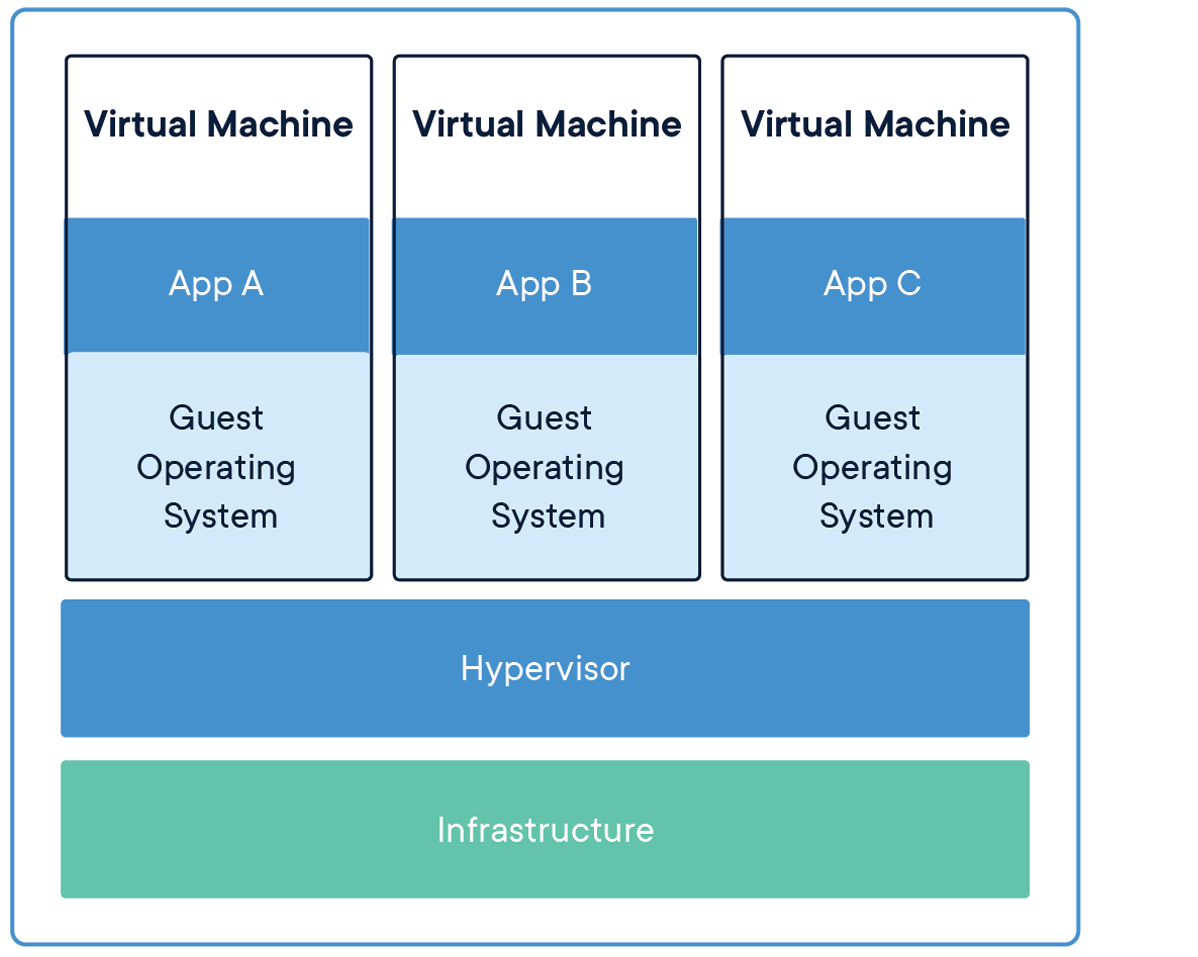
\includegraphics[width=0.5\linewidth]{vm_arch.png}
                    \caption[VM Setup]{Image portraying the general architecture of a VM-oriented setup. \cite{bib:vm-setup-img}.}
                    \label{fig:vm-arch}
                \end{figure}

            \subsubsection{Containers} \label{sec:container-intro}
                Before beginning to discuss whether containers are suitable for our purpose, we should begin by describing what a \textit{container} really is as it can be a confusing actor in the virtualization realm. Please note this section has been purposefully written as a high-level description of container technology. As stated before, a more technical discussion is presented on section \ref{sec:container-techy} belonging to chapter \ref{chap:2}.\\

                According to docker's documentation \cite{bib:docker-doc}, ``a \textit{container} is a standard unit of software that packages up code and all its dependencies so the application runs quickly and reliably from one computing environment to another''. Now, this definition is a perfect representative of the main kind of problems we will have to face when trying to bend containers to our will throughout the development process. Containers are designed to try and increase the portability of applications. In today's Internet-centric society, where we all want uninterrupted services, it is critical to be able to change an application's environment at a moment's notice due to outages, ending support cycles for software, security breaches... That is why the container technology has developed at such a high pace. It provides the infrastructure for a reliable service delivery. Now, we could ``twist'' the definition if we were to think of applications as full-fledged operating systems. That is, if we run a whole OS within these containers we would be actually achieving our goal: each container will behave as a network node so, in other words, we would only need to cope with $36$ concurrent containers: an easier task than doing the proper thing with VMs.\\

                One of the questions we asked ourselves when trying to decide on a technology was: what makes a container different than a VM? If we go back to the section we devoted to virtual machines we will notice how they run a full-fledged operating system as a guest. This implies each VM has its own \textit{kernel}. This is clearly shown on figure \ref{fig:vm-arch}.\\

                Kernels and their design have been the topic of many books and documents. We just need to know that the \textit{kernel} is the piece of software ``gluing'' the hardware and user-land software (programs such as browsers) together. That is, it allows applications to access the computing resources in an organized manner, enabling the sharing of resources amongst them. As we are telematics engineers we usually find the \textit{kernel} concept easier to understand in terms of the abstractions it offers us; the network socket being the most familiar. Through it, our applications can leverage the networking capabilities of the machine they're running on for instance.\\

                Unlike VMs, containers all share a single \textit{kernel}. We can then think of containers as a way of isolating applications along with all their dependencies within a shared computing platform. We don't need ``specialized'' software agents such as an hypervisor; we would only need to be very meticulous and know the \textit{kernel's} offered facilities very well to achieve the end result offered by containers. Projects like \textit{bocker} \cite{bib:bocker} prove one can achieve similar results to the ones provided by docker if only interested in a subset of the latter's capabilities. Nonetheless, one can regard containers as light VMs throughout the development as, even though it is not exactly true, it won't hinder our development approach. Figure \ref{fig:container-arch} shows the overall architecture of a container-based approach. Comparing it to figure \ref{fig:vm-arch} can be truly revealing when comparing both virtualization approaches.\\

                \begin{figure}
                    \centering
                    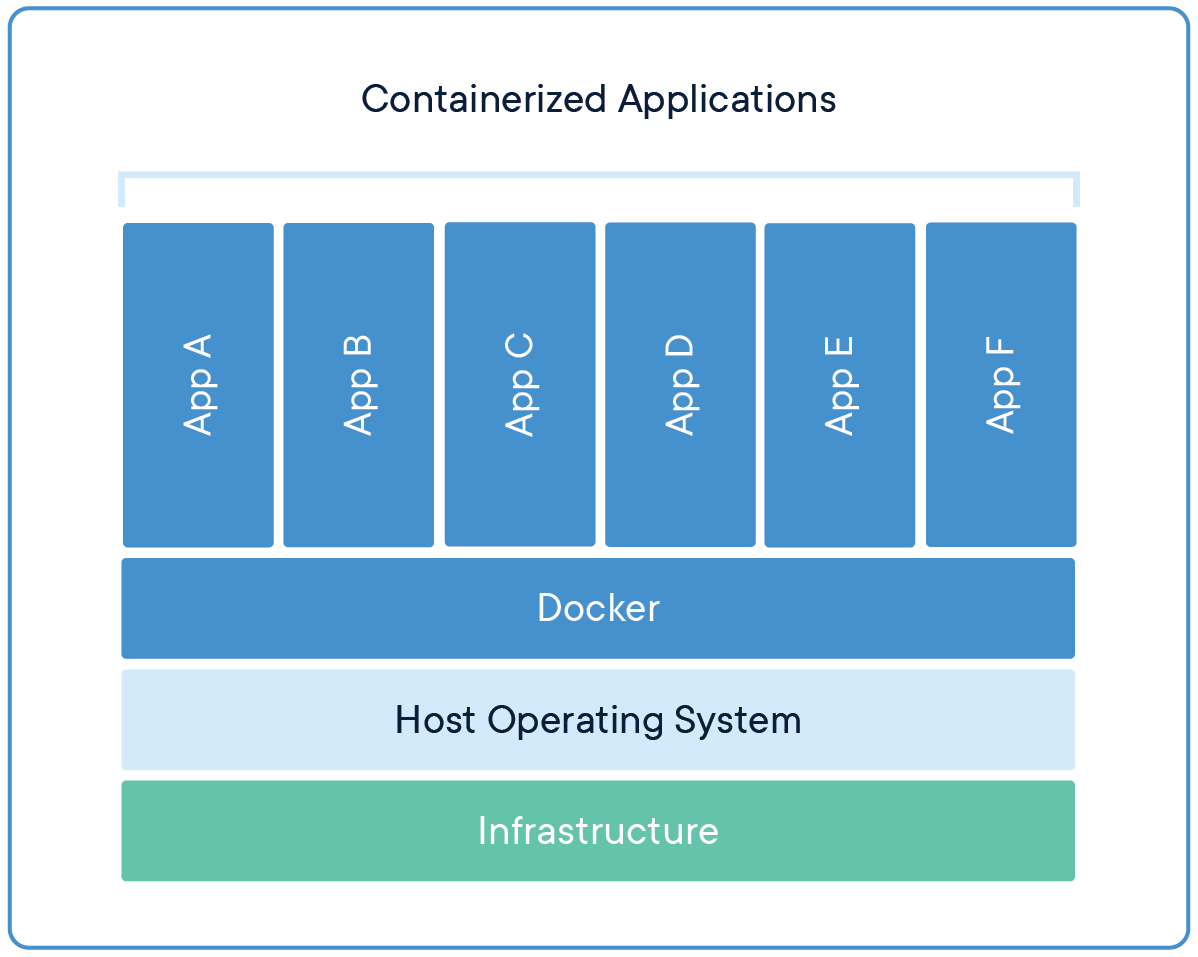
\includegraphics[width=0.5\linewidth]{container_arch.png}
                    \caption[Container Setup]{Image portraying the general architecture of a container-oriented setup. \cite{bib:container-setup-img}}
                    \label{fig:container-arch}
                \end{figure}

                \paragraph{Containers and Docker}
                    Container technology can be thought of as a standard. However, the way that technology is implemented can vary. Then, docker offers an \textit{implementation} for containers. This is a similar situation to that of VMs. The idea of a virtual machine has found two main implementations by VirtualBox and VMWare. This concept is similar to the situation posed by RFCs published by the IETF. They propose a standard and several people try to implement it according to their coding style, level of knowledge...

                    If we are to be entirely correct when it comes to nomenclature we would have to say that our solution is going to be based on docker's \textit{container implementation}.\\

                On top of container technology being lighter than that of VMs, which makes it more scalable, we also found the amount of documentation regarding the network infrastructure to be much larger. That gave us a strong foothold in our path to getting our framework up and running. Another positive aspect on containers we initially considered was the existence of \textit{container orchestration tools} such as \textit{Kubernetes} which we thought could make our job easier. We'll devote a few paragraphs to discussing why, in the end, \textit{Kubernetes} wasn't that much of a fit for us.

            \subsubsection{Kubernetes}
                As stated in \textit{Kubernetes'} own documentation \cite{bib:kubernetes-doc}, ``\textit{Kubernetes} is an open source container orchestration engine for automating deployment, scaling, and management of containerized applications''. In other words, \textit{Kubernetes} let's us define how we want our application to behave through a manifest provided in a \texttt{*.yaml} formatted file. Now, if we consider docker to be focused on offering ``services'', \textit{Kubernetes} takes that objective to the next level. It's a product aimed at professionals that's engineered to be stable. That means that meddling with the internals in an effort to achieve our goals was bound to be an extremely difficult task. By employing \textit{Kubernetes} we would be using an infrastructure that's already been laid for us, which is difficult to change and that does not behave how we want it to. We believe using a tool only to work against its basic principles is a wrong approach. That's why we decided to manually build the needed infrastructure from the ground up starting from docker containers.\\

                Just to give a concrete example of what we mean by working against the pre-existing infrastructure we could take a look at how \textit{Kubernetes} connects nodes. As it needs to offer some kind of service it will set up the internal network topology in such a way that all the nodes are able to connect among themselves. Given our requirement of implementing a firewall in the topologies we need to be working with, we can conclude it would be cumbersome to try to implement a firewall in an infrastructure whose primary concern is enabling communication links amongst all the network nodes. It's this diametrically opposite approach that made us dismiss \textit{Kubernetes} as a feasible solution.\\

        \subsection{Getting the Operating System}
            After settling on an option providing the ``hardware'' our software is to run on, we need to decide which operating system is the best suited for the task we have been proposed. Given today's ecosystem we quickly thought of the three main contenders in the user market. These are \textit{Microsoft Windows}, \textit{macOS} and \textit{Linux}. Before delving any deeper into the discussion about which to employ we would like to clarify our choice of words when referring to the last option.\\

            \paragraph{Linux vs. GNU/Linux}
                Strictly speaking, Linux is just the kernel of Linux-based distributions or \textit{distros}. As we explained in the previous section, a kernel is the piece of software gluing the hardware and user software together. It accomplishes this non-trivial feat by offering applications an interface through which they can request services. This kernel will then fulfill these requests in an orderly manner so that applications can coexist and cooperate towards a better overall usage of the system. These applications can in fact not even be aware that they are running alongside others.

                The kernel is for many the most crucial piece of software within a full fledged operating system. It's the cornerstone on which everything else is built. Nonetheless, if a non-technical user were given just a kernel they would have a very hard time making any use of it. This is where applications or user programs come into play. The make use of the OS's services and they let an end-user get meaningful work done. These end user programs range form text editors such as \texttt{vim} or \texttt{Microsoft Word} to VoIP (Voice over IP) PBXs (Private Branch eXchanges) like \texttt{asterisk}.

                The role of GNU in all this is providing many of these end user programs as free (as in freedom) software. Huge projects like the \texttt{gnome} desktop environment and \texttt{make} (which we are using for compiling this \LaTeX file) carry the GNU stamp. Given the above, GNU argues operating systems packaging their tools should be considered GNU/Linux systems as these two terms work cooperatively, i.e. they are software pieces with distinct purposes. While we consider this to be absolutely true for end-user systems such as \texttt{Ubuntu desktop} and \texttt{Debian} we feel this is not the real case with us.

                We will be running our network nodes as docker containers and we will try to make the image ran by these containers as lightweight as possible. In doing that we will only rely on GNU's shell, \texttt{bash}, for running a very restricted collection of commands. That is why we will refer to our platform as Linux containers instead of GNU/Linux ones.

            Knowing we have already restricted ourselves to the use of container technology we can discard \textit{macOS} as an option right away as there is no official support for it. We could have used \textit{Windows}-based containers but given our uncommon requirements we opted to use a \textit{linux}-based one. Given we feel comfortable with it, we settled on using \textit{Ubuntu} docker images for running our nodes. The version we employed during the testing phase was deemed \texttt{Bionic Beaver} and had version number \texttt{18.04 LTS} (Long Term Release) which boasts a higher stability than yearly versions. Given our requirements, all our work should run ``just fine'' on newer versions. We nonetheless recommend working to \texttt{LTS} releases as the yearly builds can sometimes behave unexpectedly. On top of our choice's flexibility, we mustn't forget about the price and licensing factors. Even though we haven't looked into these topics regarding Microsoft's OS, Windows licenses tend to be more restrictive than those attached to Ubuntu. As we plan on working at a very ``low level'' with the kernel's internal network infrastructure we aren't entirely sure if that would be allowed by Window's license terms. On top of that Ubuntu doesn't cost anything, so we won't have to be concerned about a monetary budget. Putting it all together justifies why we decided to run Ubuntu within our own containers.


    \chapter{Used Technology Analysis}
    According to the discussion in the previous chapter we have settled on docker containers running Ubuntu for providing the backbone of our virtualized networks. Now, once we are clear so as to what technology to employ we need to get down to the nitty gritty of implementing a full-fledged virtual network infrastructure. In order to do so we need to become acquainted with the Linux kernel.

    \section{Enter the Network Stack}
        A fascinating but rather messy image is \href{https://upload.wikimedia.org/wikipedia/commons/5/5b/Linux_kernel_map.png}{Linux's "Map"}. If we pay close attention we'll see how one of the columns is just devoted to networking. The software entities comprising this column is what we will refer to as \textit{Linux's Network Stack}\\

         The word stack is something that shows up time and time again in the area of networking. It helps us have a top-level view of how logical entities cooperate within a network. When we think about stacks we naturally begin to consider them in terms of the layers composing them with each layer tackling a simple task and offering services to the layer above whilst using those provided by the layer below. It's not going to be any different with Linux; we can think of its network stack as a huge "blob" of code which all network packets reaching a Linux-based system traverse. Thus, if we can alter how Linux processes packets or build "virtual" connections between different network stacks we would be capable of constructing a de-facto virtual network tailored to our needs.\\

         \paragraph{Naming Packets}
            Before we go on we need to shed some light on the naming we are going to use regarding the units of data exchanged through network links. Even though the term packet tremendously generic we feel it's not a wrong one to turn to in our case. When we wire up several network nodes together we are looking for full connectivity, that is, connectivity at the application level. Thus, we are not really that interested on what layer the "packet" is at, we don't really care if the packet is a \texttt{segment}, \texttt{datagram} or \texttt{frame}. In the case a need for more specific naming turns up we won't hesitate to use it but we prefer to keep the writing simple and avoiding getting bogged down with technicalities where we feel the benefit is not that obvious.

            A prime example of the above would be the use of the term \texttt{packet} instead of \texttt{link-layer frame} in the section's introduction. \texttt{Frame} is the correct term for referring to the data structure a \texttt{NIC} (Network Interface Card) hands to the kernel (albeit somewhat processed as the preamble and Frame Check Sequence of Ethernet frames are usually stripped from incoming frames by the \texttt{NIC} itself as seen \href{https://gitlab.com/wireshark/wireshark/-/wikis/Ethernet}{here}).

        If we think about network stacks, we would probably believe we need to have one per machine. That is, every network-capable devices must have their own \textit{data-path} which packets are to traverse. What may not be so simple is thinking that a machine \textit{may} have more than one network stack. In order to get a firmer grasp on the implications of the above idea let's revisit the world of network interfaces.\\
        
        When we first started learning about network architectures we where boggled by the fact that a machine could have more than one NIC. This implied it had several different IP addresses "attached" to it which provided redundancy amongst other several capabilities like traffic control. What astonished us the most was the raw power of not imposing a limit on the number of NICs a machine could have. That simple fact allowed routers to exist for instance and you could do "silly" stuff such as getting a packet through an interface and \texttt{echoing} it out the other. All in all, it provided loads of flexibility to the whole system.\\

        Now, if we transpose the above to the concept of network stacks we could be talking about packets being interchanged in between them whilst residing on the same machine nonetheless. If we sit back and take a look at the larger picture we can clearly see that packet exchanges below the application level are logically exchanged between network stacks belonging to different machines as it's the stack who's in charge of processing said data structures. Seeing matters in that light and knowing we can have several network stacks on a single platform, talking about packets being interchanged within a machine doesn't seem that far fetched now.\\

        Given the previous discussion we can now clearly see the base on which everything else is built upon. The ability to have several coexisting network stacks on a machine and being able to connect them as we please is such a powerful tool that our work is only scratching the surface of the capabilities enabled by this kind of technology. Linux's network stacks are nothing short of an ode to code modularity if you ask us.\\

        All the previous discussion is related with the theoretical or conceptual realm of matters. We will now delve into how we can translate these ideas into a working virtual network. After going through that process we'll also look into how we decided to do everything manually once we have a broader technical background on the subject.\\

        Finally, we feel we need to clarify that, even though it may be clear at this point, all the network traffic we are to generate originates from within our own system. In other words, our network would be perfectly capable of working without any Internet access.\\

    \section{The Network Namespace}
        % \pyfile{Code_snippets/foo.py}

        % Just as we have previously discussed, design and implementation are two very different things. A prime example is the case of the \texttt{SNMP} tools where \texttt{SNMP} stands for \texttt{Simple Network Management Protocol}. This protocol was originally defined in \href{https://tools.ietf.org/html/rfc1067}{RFC 1067} but no implementation was defined. With time, the \texttt{net-snmp} suite of tools became the de-facto implementation for \texttt{SNMP}. It is then of the utmost importance to notice that the design and implementation needn't be carried out by the same people; in fact, it's not uncommon to have several implementations for a given design. That's the case with shells of which we have so many, \texttt{bash}, \texttt{zsh}, \texttt{ksh} and so on. Then, we can expect the Linux...\\

        Many of the programming languages dominating today's market are object oriented. This, very roughly, means that the programmer is expected to generate \textit{classes} representing "real-life" entities to some extent. These classes are defined by their \textit{attributes} (characteristics) and their \textit{methods} (what they can do). Now, a class by itself cannot do anything, we need to \textit{instantiate} it so that we create an \textit{object} of that class. We'll then be capable of using the newly created object as we please.\\

        This concept on instantiation is actually quite powerful as it appears continuously in many areas of engineering. Now, we could say that Linux's network namespaces work in a similar fashion to classes. We can think of the network stack as the class and what we call \textit{network namespaces} as the objects. Let's delve a bit deeper into what these namespaces really are.\\

        As seen \href{https://en.wikipedia.org/wiki/Linux_namespaces}{here}, namespaces are not only seen when doing networking stuff, they are a feature of the Linux kernel employed in many other areas. These namespaces let us partition kernel resources so that each process sees a resource that's only for it, it's not shared. When applied to networking we can see how each network namespace represents an entire network stack. Then, if we set up several network namespaces (namespaces from now on as this is the only type of namespace we will deal with) we have effectively housed several network stacks under the same roof. If there was any way of interconnecting these namespaces we would have taken quite a dent off our task.\\

        We will now take a look at the virtual wires we have fought so many times against, the so called \texttt{veths}.\\

    \section{Wire time}
        In a previous section we already provided some comments on what NICs are. Knowing that interfaces create "bridges" between different systems we can clearly see how these network interfaces bridge digital systems to a communication network; they let these digital machines leverage the communication capacities of computer networks.\\

        Whilst almost all engineers could recognize what a NIC physically is, the matter is not that simple regarding how the OS treats these interfaces. We find it quite helpful to think of what we would do if we had to implement some software solutions that had to employ network's capabilities. There must be a "way" that these hardware components can be used from the application perspective, that is, the OS needs to offer some kind of abstraction through which we can make use of the NIC itself. This abstraction is what we will call a OS-level NIC or network interface.\\

        Before delving any deeper into this matter we need to discuss what the \texttt{iproute2} suite is as we believe adding some examples to the contents to follow would really enrich them.

        \subsection{Meeting \texttt{iproute2}}
            The time we spend on terminal emulators has exponentially increased as we worked our way through our bachelor's. Even though they provide quite a fast way to "get around" the computer they can be a little abstract at times. We are always aware that the OS "under" us has many running processes and provides us with services that can be used at our request. The thing is, faith can at times be scarce so we usually have tools that can inform us about what's going on "behind the scenes". This is the case for programs like \texttt{ps} which reports the status of the system's processes or \texttt{w} which tells us about who is currently logged on the system as well as what they are up to. When using a shell we are aware of the fact that other processes are running and that other users may be logged on but we nonetheless have tools that let us consult the current status of the system.\\

            Where networking is concerned, \texttt{iproute2} is like a Swiss Army Knife. It's a \textit{suite} or collection of tools that lets us do everything from inspecting the current interfaces and routes to generating \texttt{IPv6/IPv4} tunnels. We'll only be concerned with the \texttt{ip} command in our case which is in charge of "showing / manipulating routing, network devices, interfaces and tunnels" as seen in \texttt{ip}'s manpage (which can be consulted with \texttt{man ip}).

    \chapter{Manually Bringing Up a Simple Network} \label{chap:3}
    \epigraph{If the vendors started doing everything right, we would be out of a job.
    Let's hear it for OSI and X!  With those babies in the wings, we can count
    on being employed until we drop, or get smart and switch to gardening,
    paper folding, or something.}{\textit{C. Philip Wood}}

    Figure \ref{fig:sample-topology} showcases a simple topology we will instantiate by applying the contents described in chapter \ref{chap:2}. Instead of relying on our framework to perform the task, we will manually carry out all the needed steps and detail them in a code listing. This demonstrates how are tool is nothing more than an additional ``layer'' in charge of managing the subtleties we will manually deal with once the topologies' complexity begins to increase.\\

    \section{A Note on the Chosen Private IP Range}
        As seen on section $3$ of \cite{bib:rfc1918} we could have chosen private addresses within one of $3$ private network address spaces. Doing so guarantees we will not run into any collisions should we want to let our virtual hosts and routers communicate with the public Internet. We should nonetheless be aware of the fact that, if we are pursuing a completely isolated virtual network we need not adhere to these reserved address ranges: no collisions could probably occur.\\

        Given we did not have a firm reason not to choose one of the reserved private address spaces, we decided to make use of them. As our home network uses the \textit{192.168.1.0/24} range and, in our experience, the \textit{172.16.0.0./12} space tends to be more common, we decided to assign addresses within the \textit{10.0.0.0/8} pool. These are the ones that will be included in any figures and listings that need to explicitly include IP addresses.\\

    \begin{figure}
        \centering
        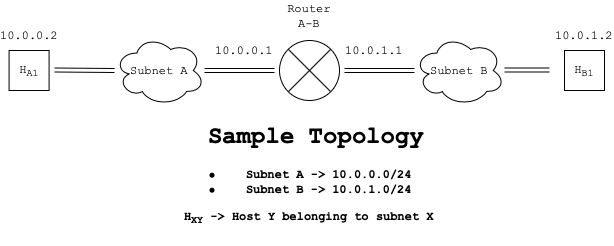
\includegraphics[width=\linewidth]{sample_topology.png}
        \caption[A Sample Topology]{The Sample Topology We Will Set Up Throughout Chapter \ref{chap:3}.}
        \label{fig:sample-topology}
    \end{figure}

    \section{Automating the Sample Topology}
        Listing \ref{lst:sample-topology} contains the shell script automating the deployment of the network showcased on figure \ref{fig:sample-topology}. The script itself contains messages that are to be printed to the user which clarify its operation to a great extent.\\

        \subsection{Running the Script}
            As seen on \textit{line 1} of listing \ref{lst:sample-topology} this script is to be tun within a \textit{bash} shell. This can be accomplished in one of two ways as shown on \ref{lst:bash-script}. As we will later look into, the script is to be run by \textit{root} so that it can carry out the needed operations. This amounts to prepending the command we choose to run the script by \texttt{sudo}.\\

            \begin{lstlisting}[language = bash, caption = Running a \textit{bash} Script., label = lst:bash-script]
                # Making the script executable and running it.
                chmod +x <script-name> && sudo ./<script-name>

                # Spawning a privileged shell and running the script in it.
                sudo bash <script-name>
            \end{lstlisting}

        \subsection{Checking the Script is Run by root}
            The privileged user in \textit{UNIX}-based systems is identified by a \textit{UID} (User ID) of $0$. When a program is run, the associated process will have the \textit{UID} of the user who launched it. Some program's permissions allow it to run with a different \textit{UID} than that of the user executing it: this is wha we call the \textit{EUID} (Effective \textit{UID})). In any case, if the \textit{EUID} of a process evaluates to $0$ it is being run by \textit{root}. This is what is being checked by \textit{lines 3-7} on listing \ref{lst:sample-topology}. If the user running the script is not \textit{root} we will simply abort execution whilst warning the user.\\

        \subsection{Automatically Tearing Down the Topology}
            As seen in \textit{lines 9-17}, the script shown on listing \ref{lst:sample-topology} is prepared to dismantle the network topology it brings up when invoked a second time. The trigger for this behaviour is passing a parameter when running the script. Any parameter will cause the removal of the entire virtual network: this is not the best practice when writing code but it simplifies handling the arguments passed to the script. We are concerned with clearly portraying the technologies discussed in chapter \ref{chap:2}, not with teaching the user how to write proper shell scripts. In any case, running \texttt{sudo bash <script-name> quit} will dismantle the sample virtual topology.\\

        \lstinputlisting[language = bash, caption = Automatic Deployment of the Sample Topology., label = lst:sample-topology]{Code_snippets/sample_topology.sh}

    \section{Testing the Topology Is Working}
        Once the script shown on listing \ref{lst:sample-topology} has been run we should have a full-fledged virtual network at our disposal. The simplest way to check we do have full connectivity is checking one of the hosts can ``see the other''. we can accomplish our objective by running a shell within one of the hosts and then trying to \textit{ping} the other. We can extract the appropriate \textit{IP} addresses from figure \ref{fig:sample-topology}. Listing \ref{lst:sample-topology-test} shows how we can open up a shell within host $H_{A_1}$ and launch \textit{ping} against host $H_{B_1}$.\\

        \begin{lstlisting}[language = bash, caption = Testing the Sample Topology., label = lst:sample-topology-test]
            # Spawn a shell within H-A-1
            docker exec -it h-a-1 bash

            # Ping H-B-1 3 times from H-A-1
            root@h-a-1:/$ ping -c 3 10.0.1.2

            # It should produce an output similar to:
                # PING 10.0.1.2 (10.0.1.2) 56(84) bytes of data.
                # 64 bytes from 10.0.1.2: icmp_seq=1 ttl=63 time=0.036 ms
                # 64 bytes from 10.0.1.2: icmp_seq=2 ttl=63 time=0.057 ms
                # 64 bytes from 10.0.1.2: icmp_seq=3 ttl=63 time=0.062 ms
                #
                # --- 10.0.1.2 ping statistics ---
                # 3 packets transmitted, 3 received, 0% packet loss,\
                    # time 2049ms
                # rtt min/avg/max/mdev = 0.036/0.051/0.062/0.011 ms

            # We can also run traceroute
            root@h-a-1:/$ traceroute 10.0.1.2

            # It should produce an output similar to:
                # traceroute to 10.0.1.2 (10.0.1.2), 30 hops max, 60\
                    # byte packets
                # 1  10.0.0.1 (10.0.0.1)  0.029 ms  0.039 ms  0.007 ms
                # 2  10.0.1.2 (10.0.1.2)  0.018 ms  0.023 ms  0.041 ms
        \end{lstlisting}

    Now that we have shown how to ``manually'' set up a simple network we begin to discover the challenges that will surely arise as their complexity grows. What is more, we also need to add additional functionalities such as moving end nodes around the network in a way that does not mangle the network's operation. The next chapter is devoted to providing a high level overview of our tool's design and operation together with a comprehensive collection of the actions it can and cannot perform.

\end{document}